\chapter{Фрагменты исходных текстов программ}\label{app-format}

\lstinputlisting[
label=lst:Visualization,
frame=lines,
language=python,
caption=Листинг процедуры визуализации
]{listings/vis.py}

\lstinputlisting[
label=lst:Training,
frame=lines,
language=python,
caption=Листинг процедуры обучения
]{listings/train.py}

\lstinputlisting[
label=lst:Gen,
frame=lines,
language=python,
caption=Скрипт для генерации набора данных
]{listings/get_dataset.py}

\chapter{Рисунки и Иллюстрации}\label{morefigs}

\begin{figure}[h]
	\centering
	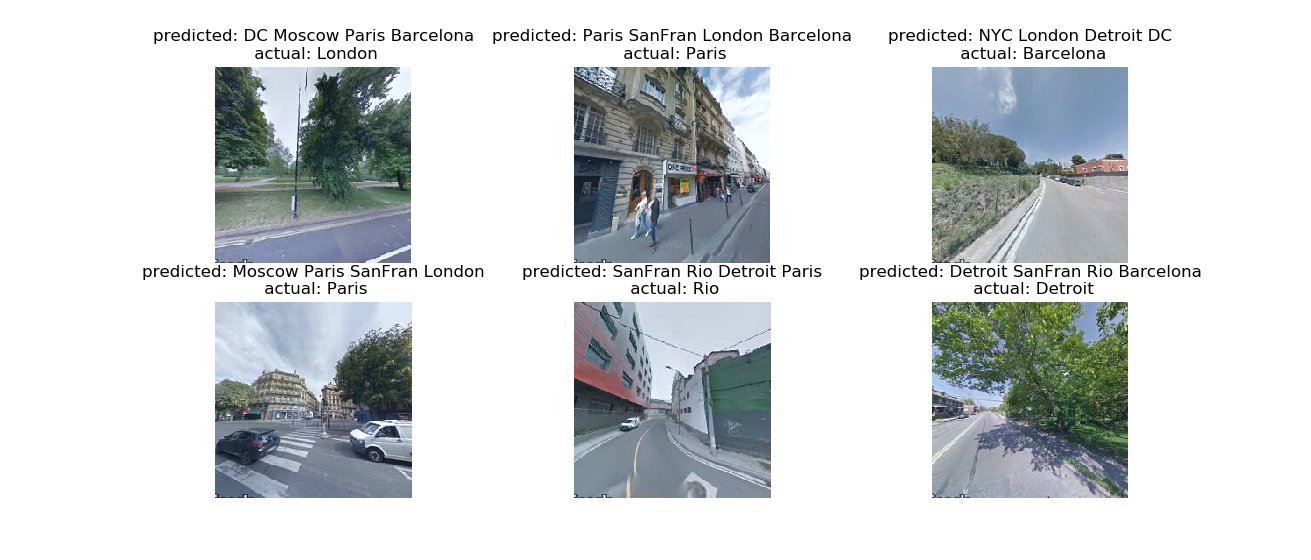
\includegraphics[width=0.9\linewidth]{img/add_vis}
	\caption{Дополнительная визуализация для случая с 1 фотографией}
	\label{fig:addvis}
\end{figure}

\begin{table}[h]
	\centering
\begin{tabu}{l|cccc}
	Класс & precision & recall & f1-score & support \\ \hline
	Barcelona        &   0.35    &  0.32  &   0.34   &   100   \\
	DC               &   0.51    &  0.36  &   0.42   &   100   \\
	Detroit          &   0.57    &  0.70  &   0.63   &   100   \\
	London           &   0.46    &  0.46  &   0.46   &   100   \\
	Moscow           &   0.36    &  0.48  &   0.41   &   100   \\
	NYC              &   0.47    &  0.29  &   0.36   &   100   \\
	Paris            &   0.30    &  0.31  &   0.31   &   100   \\
	Rio              &   0.45    &  0.43  &   0.44   &   100   \\
	SanFran          &   0.46    &  0.49  &   0.48   &   100   \\
	Sydney           &   0.54    &  0.63  &   0.58   &   100   \\
	avg / total      &   0.45    &  0.45  &   0.44   &  1000   \\\hline
\end{tabu}
\label{tbl:clsrep}
\caption{Отчёт по классификации для полностью переученной сети на валидационной выборке}
\end{table}

\begin{figure}[h]
	\centering
	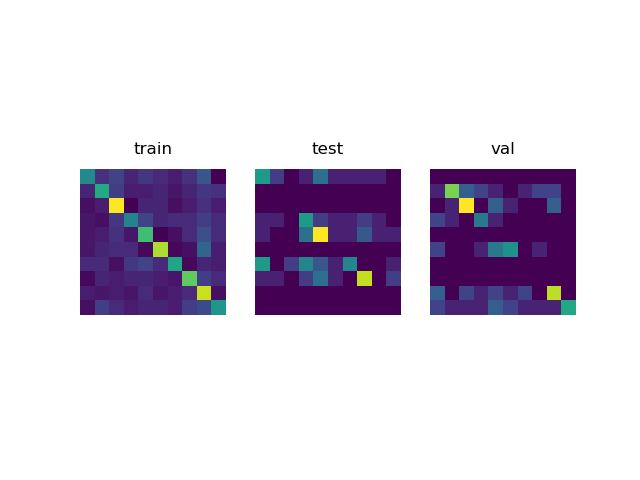
\includegraphics[width=0.7\linewidth]{img/confM}
	\caption{Матрицы неточностей для различных выборок.}
	\label{fig:confm}
\end{figure}

\begin{figure}[h]
	\centering
	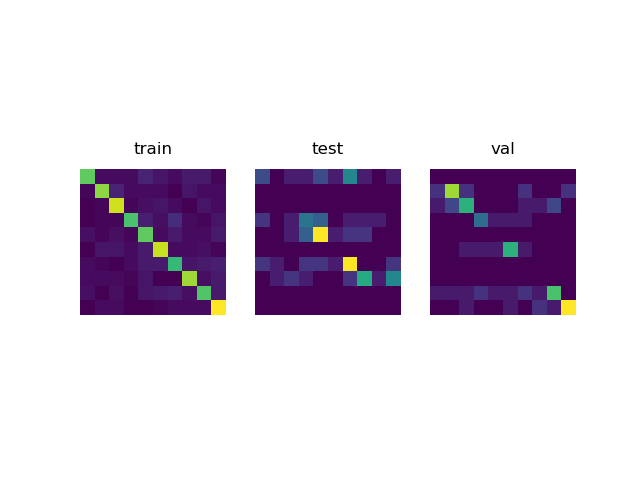
\includegraphics[width=0.7\linewidth]{img/confM2}
	\caption{Матрицы неточностей для различных выборок для полностью переученной сети }
	\label{fig:confm2}
\end{figure}
